\chapter{TurtleBot Gazebo Simulation}
\label{chap:TurtleBotGazeboSimulation}

	
\section{.bashrc}
	\texttt{export TURTLEBOT\_STACKS = ninja-hexagons}
	\\
	\texttt{export TURTLEBOT\_3D\_SENSOR = ninja-kinect}
	\\
	\texttt{export GAZEBO\_MODEL\_PATH}


\section{Starting Gazebo simulation}

\texttt{roslaunch turtlebot\_bringup simulation.launch}
	
	Starts Gazebo, the map server and the robot	
	\\	
	\\	
		
\texttt{roslaunch turtlebot\_bringup navigation\_gazebo.launch}
	
	Starts amcl move\_base
	\\
	\\
	
\texttt{roslaunch rviz\_sim.launch}
	
	Starts local cost map

\section{topics}

\texttt{/leonardo/move\_base\_simple/goal}

	to publish the robots destination
\\
\\
\texttt{/leonardo/initialpose}
	pose estimate	


\section{Turtlebot Sensor Plugin}

To simulate various Scenarios using the Turtlebot there was a need for a more specific and configurable type of sensor. We developed a sensor plugin for gazebo to accomplish that. It allows the user to configure detection angles, range and the type of object in a configuration file. 

\subsection{Configuration}

The configuration format uses a similar syntax as the configuration for the ProcessManager mentioned in a previous section of this document.

The file itself is located at the configuration path (usually \textit{~/ttbws/cnc-turtlebots/etc/}) and has the filename \textit{LogicalCamera.conf}.

Let's take a look at the following example configuration:

\begin{verbatim}
[LogicalCamera]
        [Victim]
                # meter
                range = 3
                type = victim
                # Hz
                publishingRateHz = 1

                # angles have to be set from 180 to -180 degree
                [DetectAngles]
                        [Front]
                                startAngle = -135
                                endAngle = 135
                        [!Front]
                [!DetectAngles]
        [!Victim]
        [Fire]
                # meter
                range = 5
                type = fire
                # Hz
                publishingRateHz = 10

                # angles have to be set from 180 to -180 degree
                [DetectAngles]
                        [Front]
                                startAngle = -180
                                endAngle = 180
                        [!Front]
                [!DetectAngles]
        [!Fire]
[!LogicalCamera]
\end{verbatim}

The first Block \texttt{[LogicalCamera]} is the uppermost block and has to be followed by \texttt{[!LogicalCamera]} at the end.

In this example we want to detect two types of objects. The first one is the presence of victims and the second one is fire. Each distinct type has to be defined as a block, similar to the uppermost LogicalCamera Block. Hence we have \texttt{[Victim] ... [!Victim]} and \texttt{[Fire] ... [!Fire]} here.

In these type blocks, we now have to define the properties of the sensor for that given type of object.

Here, a victim can be detected in a \textbf{range} of 3 meters, as given to  the range parameter.

The \textbf{type} parameter is used by the plugin to determine which object belongs to which type. The plugin filters these types depending on the objects name in gazebo. So an object called \textit{victim\_box} is going to be detected as a victim type object.

Using the parameter \textbf{publishingRateHz} as the name suggests you can set the rate in which an object may be detected. A victim will be only detected once a second, while a fire can be detected up to ten times a second.

Next, the block \textbf{DetectAngles} allows you to specify multiple sections in which the robot can detect the object.

Anlges have to be in a range from -180° to 180°.

The following picture clarifies, how the angles have to be speciefied:

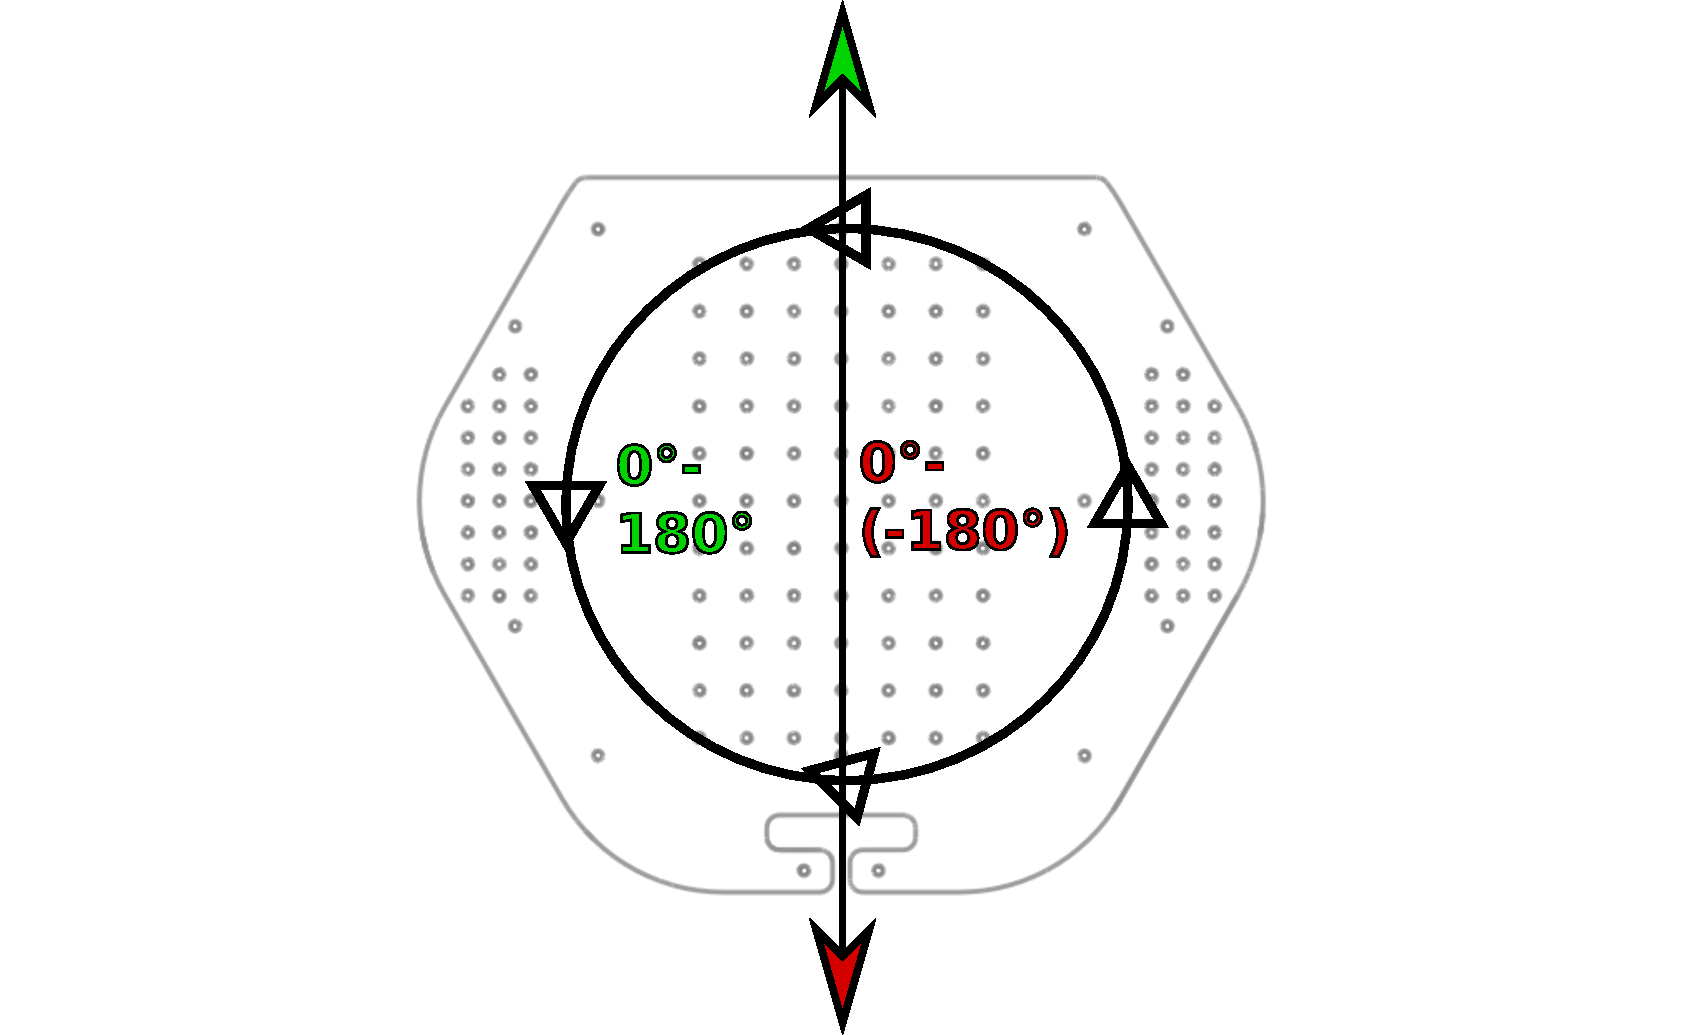
\includegraphics[width=1.0\textwidth]{ttbangles.pdf}

\subsection{Sensor message}

Every time an object has been detected according to the configuration, a ROS message gets sent.

The name of the ros topic is \textit{logical\_camera} and is namespaced with the robot name, as configured in the \textit{robot.simulation} file. So for a robot named leonardo, the message will get published on the topic  /leonardo/logical\_camera.\\

The message itself has the following fields:

\texttt{string modelName}

	Name of the detected model/object in gazebo

\texttt{geometry\_msgs/Pose2D pose}

	Posoition of the object on the x,y plane(map seen from top)

\texttt{ObjectSize size}

	Approximate size of an object. Contains fields xsize, ysize and zsize.

\texttt{time timeStamp}

	Time, when the object was detected.

\texttt{string type}

	Object type. See Configuration Section for details.

\newpage
\subsection{Robot coordinate system}

Looking from the top at the turtlebot, the coordinate system looks like that:

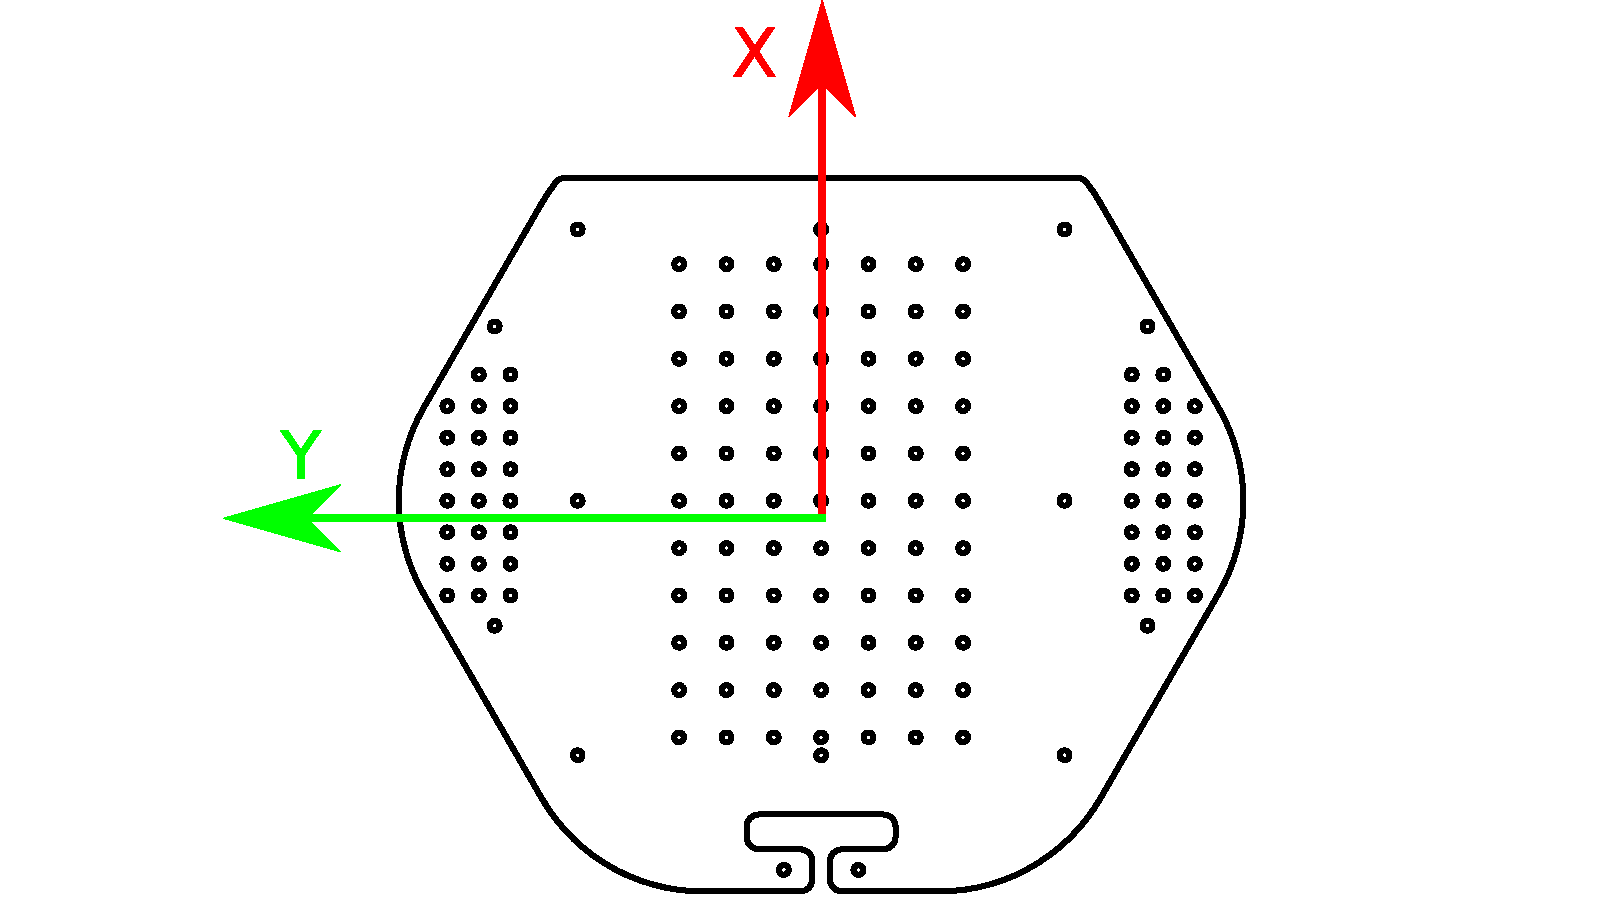
\includegraphics[width=1.0\textwidth]{ttbtop.pdf}

So the a positive X coordinate means, an object is ahead of the robot, while a negative one means, it is behind the robot. In the same way, a positive Y means that an object is detected left of the robot, while a positive Y coordinate means that it was detected on the right side.

As a side note, the Z coordinate tells you how high is an object in relation to the sensor. A positive Z means, that the object is above the sensor, while a negative Z means, that it is negative.

\subsection{Using the sensor plugin in gazebo}

First, make sure you configured the plugin as described in the configuration section.

Then simply launch gazebo using the simulation launch file:

\begin{verbatim}
roslaunch turtlebot_bringup simulation.launch
\end{verbatim}

In order for the plugin to correctly detect and filter the objects, you have to give each object a name, that contains the type string from the configuration. A \textit{victim\_box} may for example be detected  as a victim or box type of object.

Now, to add objects in Gazebo you can for example add a cube using the cube button in toolbar on top of the 3D view. For more information about adding objects in gazebo, take a look at the corresponding gazebo tutorial.

To quickly test the sensor you can add a cube or sphere and rename it as follows.  First, add an object using the cube, sphere or cylindar button in the top bar. Then select the object by left clicking on it and then right click it to bring up the context menu. In the menu select \textit{Edit Model}. You are now in the Model Editor. In the left Pane select the Model Tab and change the Model Name to a name that contains the type string. After you are done, exit the Model Editor by select \textit{Exit Model Editor} in the \textit{File Menu}.

Now you may have to continue the simulation by pressing the play button on the bar below the 3D view. After that you should be able to receive messages from the plugin on the \textit{logical\_camera} topic.